\documentclass{article}
\usepackage{graphicx} % Required for inserting images
\usepackage[english]{babel}
\usepackage{amsmath}
\usepackage{amsthm}
\usepackage{amssymb}
\usepackage[margin=.75in]{geometry}
\usepackage{hyperref}
\usepackage{amsfonts}
\usepackage{mathrsfs}
\usepackage[version=4]{mhchem}
\usepackage{bigints}
\usepackage{caption}
\usepackage{xpatch}
\usepackage{xr}
\usepackage{enumitem}

\setlength{\parindent}{0pt}
\title{Bio 338 Modeling Biological Dynamics Notes}
\author{Kyle Wang}
\date{September 2026}

\newtheorem{definition}{Definition}[section]
\newtheorem{theorem}[definition]{Theorem}

\begin{document}

\maketitle
\tableofcontents
\section{Rates of Change and Basic Modeling}
\subsection{Introduction}
State: numbers that describe variables (state variables) of interest \\
State variables: Things we care about and measure\\
State space: space of allowable values of a state variable \\ 
One thing to note is that units can affect the state space. For example, the state space for allowable temperatures in Celsius is $C\in[-273.15,+\infty)$ whereas the allowable temperatures in Kelvin is $K \in [0,+\infty)$. \\
We can express differential equations as compartment diagrams. 
\begin{figure}[htbp]
    \centering
    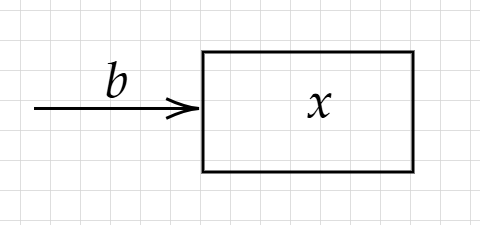
\includegraphics[width=0.5\linewidth]{linearGrowth.png}
    \caption{Compartment diagram of linear growth}
    \label{fig:linearGrowth}
\end{figure}
This diagram represents linear growth and is isomorphic to the equation 
\begin{equation*}
    \dot x=b
\end{equation*}
For these examples, let us use $x$ to describe the rabbit population. In this case, the population is increasing by $b$ rabbits per time unit (we shall say month for the example).
\begin{figure}[hbtp]
    \centering
    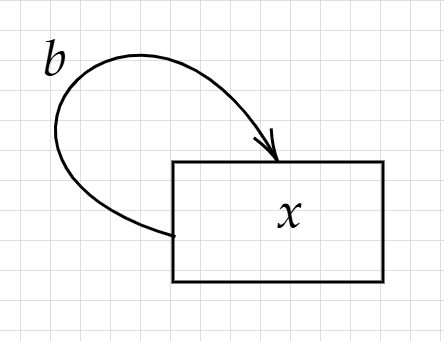
\includegraphics[width=0.5\linewidth]{perCapitaBirth.png}
    \caption{Compartment diagram of per capita growth}
    \label{fig:perCapitaGrowth}
\end{figure}
Figure \ref{fig:perCapitaGrowth} is the compartment diagram for the equation 
\begin{equation*}
    \dot x=bx
\end{equation*}
This effectively represents that more rabbits means more offspring which physically makes sense. We can adjust this model further by adding a death rate $d$. We can then draw the compartment diagram as seen in Figure \ref{fig:perCapitaBirthDeath}.
 The isomorphic differential equation for this is 
 \begin{equation*}
     \dot x=bx-dx = (b-d)x
 \end{equation*}
which has the solution 
\begin{equation*}
    x(t)=x_0e^{rt} \hspace{20pt} r =b-d
\end{equation*}

If $r>0$, then the birth rate ``out competes" the death rate which leads to exponential growth. On the other hand, if $r<0$, the death rate overrides the birth and hence the rabbit population disappears. We can make it more realistic by adding carrying capacity that only allows $k$ rabbits in our system. This system is described by the \emph{Euler-Lotka} Model 
\begin{equation*}
    \dot x = r\left(1-\frac{x}{k}\right)x
\end{equation*}

where $r$ is once again the sum of the birth and death rates. The second term effectively scales the birth and death based off of how close the population is to the carrying capacity. We must have that $r>0$ or else we see that the amount of deaths slows down as we approach the carrying capacity which is unphysical.
\begin{figure}[hbtp]
    \centering
    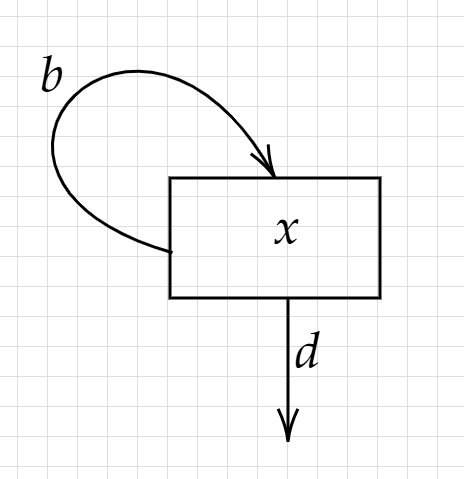
\includegraphics[width=0.5\linewidth]{perCapitaBirthDeath.png}
    \caption{Compartment diagram of per capita growth and death}
    \label{fig:perCapitaBirthDeath}
\end{figure}
If we think about when $r<0$, we also see that if $x>k$, we have unbounded growth since $r$ and $\left( 1-\frac{x}{k}\right)$ is also negative leading to $\dot x>0$ and hence unbounded growth. Even if it hypothetically did work, we wouldn't really care since $r<0$ should force everything to zero and so $k$ doesn't have any impact on our model. Checking the behavior when $r>0$, we find that if $0<x<k$, we should expect growth and indeed $\dot x>0$. When the number of rabbits is above the carrying capacity, we should expect the population to decline and indeed that occurs as $\dot x <0$.\\\\
It is also worth noting that this model assumes the number of rabbits is a continuous variable which implies fractional (or irrational) number of rabbits which is clearly not reality. We disregard this concern for large populations because the difference between 1000.5 and 1001 rabbits is trivial; however, for small populations, we would need to enforce a discrete model since the difference of one rabbit is more significant on that scale.
\subsection{Predation}
Suppose that foxes ($y$) eat rabbits ($x$). Also suppose that the rate of foxes is dependent on the food supply. We can then write the differential equation describing the number of foxes as 
\begin{equation*}
    \dot y =b[\text{food}]y-Dy
\end{equation*}
We can define the food supply as the probability of a single predation event as $p$ multiplied by the number of rabbits there are $x$. We can then multiply the food supply available by the number of wolves to feed this which hence leads to 
\begin{equation*}
    \dot y=bpxy -Dy
\end{equation*}
where $D$ is the death rate per capita for wolves. Before, we described the rabbits as just $\dot x=rx$. Now we have to factor in the deaths due to foxes which is once again the food supply multiplied by the number of foxes. We now have the set of differential equations 
\begin{equation*}
    \begin{split}
        \dot x&=rx-pxy\\
        \dot y&=bpxy-Dy
    \end{split}
\end{equation*}
And if we let all the coefficients equal 1, we get the \emph{Lotka-Volterra Model}.
\begin{equation*}
    \begin{split}
        \dot x&=x-xy\\
        \dot y&=xy-y
    \end{split}
\end{equation*}
\subsection{HIV}
What perplexed people about HIV was the timeline of the disease. The viral load would initially spike and decline within the first 8 weeks of infection. It would then stay at a low viral load for years (in what is deemed its latent phase) before slowly increasing and leading to AIDS. There were two main questions:
\begin{enumerate}
    \item What causes the initial spike and decline?
    \item What causes the sudden climb in viral load leading to AIDS?
\end{enumerate}
The initial hypothesis was that there wold be rapid viral growth and then the immune system would respond (leading to increase and decline in viral load) before replicating slowly in the background. In 1994, the first antiretroviral drugs were in clinical trials. These vaccines worked by stopping viral replication rather than directly killing existing viral particles. According to the previous hypothesis, these drugs shouldn't make a significant impact since the viruses are only replicating slowly. What they noticed was an exponential decay in viral load as time progress after the treatment. \\\\In 1996, Alan Perelson publishes \textit{HIV-1 Dynamics in Vivo: Virion Clearance Rate, Infected Cell Life-Span, and Viral Generation Time} to explain what was observed. Let us consider a basic bathtub with a faucet and a drain. The inflow is described as $Q_i$ and the outflow is described as $Q_o$ and is dependent on the volume in the bathtub. We can therefore describe the amount of volume in the bathtub, $V$ as the following differential equation 
\begin{equation*}
    \dot V=Q_i-Q_oV
\end{equation*}
We especially care about the steady state condition which is when $\dot V=0$. This leads to $V=\frac{Q_i}{Q_o}$ which effectively showed that the volume at steady state is dependent on the \emph{ratio} and not the magnitudes of $Q_i$ and $Q_o$. We could therefore have a faucet with high mass flow rate but also a really efficient drain or a dripping faucet and inefficient drain. We can't tell by solely looking at the amount of water in the drain. This extremely basic model already gives the insight that the virus is replicating extremely quickly, but the immune system is also clearing them quickly too. If we solve for $V(t)$ generally, we get 
\begin{equation*}
    \begin{split}
        \dot V&=Q_i-Q_oV \\
        \int\frac{1}{Q_i-Q_oV}dV &= t+c \\
        V(t)&=\frac{Q_i}{Q_o}+Ce^{-Q_ot}
    \end{split}
\end{equation*}
If we apply the initial condition that $V(t=0)=V_0$, then we find the constant to be $C=V_0-\frac{Q_i}{Q_o}$. If $Q_i$ and $Q_o$ are small, we should expect small exponential decay and vice versa. This effectively explains the dramatic difference the antiretrovirals made. Let us now consider a more sophisticated model. 
\begin{figure}[htbp]
    \centering
    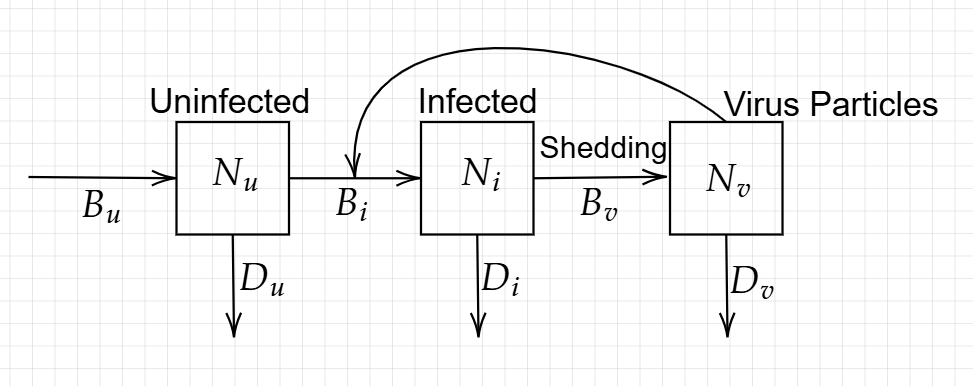
\includegraphics[width=0.5\linewidth]{HIVModel.png}
    \caption{Compartment diagram of a model similar to Perelson's}
    \label{fig:HIVModel}
\end{figure}
One thing to note is that the line from $N_v$ implies that the rate of infection is dependent on the number of virus particles. There is also a negligible consumption of $N_v$ in this process. Shedding also depends on $N_i$ but doesn't change $N_i$. We can then write these as a set of differential equations 
\begin{equation*}
    \begin{split}
        \dot N_u &= B_u-D_uN_u-B_iN_vN_u\\
        \dot N_i &=B_iN_vN_u-D_iN_i\\
        \dot N_v &= B_vN_i-D_vN_v
    \end{split}
\end{equation*}
These equations are annoying to solve analytically but we can solve it numerically. We can then graph as seen in Figure \ref{fig:HIVPlot}.
\begin{figure}[htbp]
    \centering
    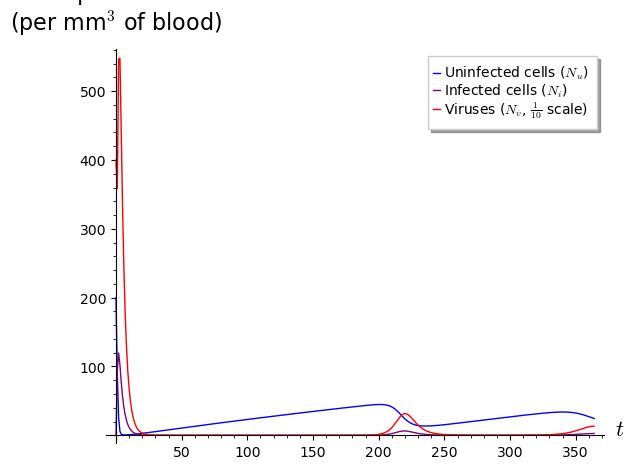
\includegraphics[width=0.5\linewidth]{HIVPlot.png}
    \caption{Plot of the amount of HIV in the blood over time with the parameters using McClain's model: $B_u=0.272, B_i=0.00027, B_v=100, D_u=0.00136, D_i=0.33, D_v=2$}
    \label{fig:HIVPlot}
\end{figure}
We can further adjust the model to include latent infected cells: that is, cells that are infected but do not shed viruses. Let us say that 10\% of cells become latently infected. Let us assume the death rate of latent cells is the same as uninfected ($D_l=D_u$). Let us also say that the latent cells become active (and begin shedding) at a rate $B_a$. Our set of differential equations is now 
\begin{equation*}
    \begin{split}
        \dot N_u &= B_u-D_uN_u-B_iN_vN_u \\
        \dot N_i &= .9B_iN_vN_u + B_aN_l -D_iN_i \\
        \dot N_l &= .1B_iN_vN_u - B_aN_l-D_uN_l \\
        \dot N_v &= B_vN_i - N_vD_v
    \end{split}
\end{equation*}
\begin{figure}[htbp]
    \centering
    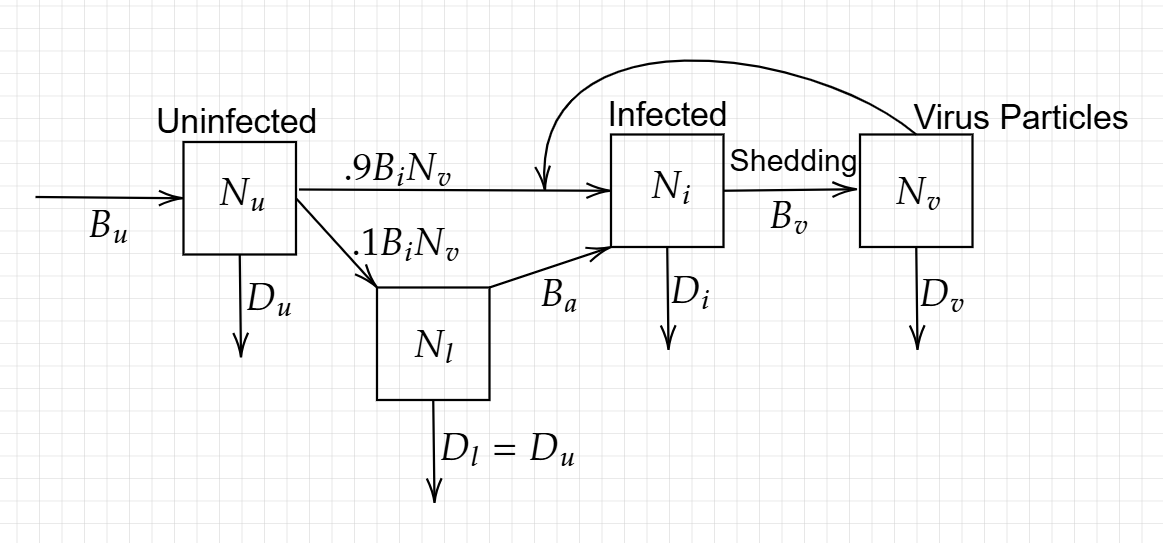
\includegraphics[width=0.5\linewidth]{McClain Latent.png}
    \caption{McClain's model including latently infected cells}
    \label{fig:McClainLatent}
\end{figure}
\subsection{Tangent Spaces}
\begin{definition}[Tangent Space]
    The tangent space of a \emph{manifold} is a vector space that contains all possible directions tangent to the manifold at that point.
\end{definition}
\begin{definition}[Manifold]
    An $n$-dimensional manifold is a topological space with the property that each point has a neighborhood that is homeomorphic to an open subset of $n$-dimensional Euclidean space.
\end{definition}
We can effectively think of the a state space as a manifold and each point on that manifold corresponds to a specific state in that state space. We can then think of the tangent spaces as all possible changes that can be made to a certain state in that state space. I wish I knew more about differential geometry but maybe G\'abor Sz\'ekelyhidi can teach me about it. 
\begin{definition}[Vector Field]
    A vector is a function $f:$ points in the state space $(\mathbb{R}^n)\mapsto$ points in the tangent space $(\mathbb{R}^n)$. 
\end{definition}
Let us look at the example $x\in[0,\infty)$ to be our state space and $\dot x=2x$ as our manifold. The state space is the positive half line and so vectors in this tangent space can point in either direction. So $-5$ or $2$ may be allowable vectors in this tangent space. However, the \emph{vector field} is strictly enforced by $\dot x=2x$ which is a \emph{subset} of the tangent space. We can also look at the vector field for the logistic model where $x\in [0,\infty)$ and $\dot x=rx\left(1-\frac{x}{k}\right),\,\,\, r>0$. We now note for $x<k$, the vector field points in the $+\hat x$ whereas if $x>k$, the vector field points in the $-\hat x$ direction. That is because there exists a fixed point at $k$.
\begin{theorem}[Banach Fixed Point Theorem]
    Let $(X,d)$ be a \emph{complete} metric space with a contraction mapping $T:X\mapsto X$. Then $T$ admits a unique fixed point $x^* \in X$ meaning $T(x^*)=x^*$. Furthermore, $X^*$ can be found as follows: start with an arbitrary element $x_0\in X$ and define $x_n = T(x_{n-1})$ for $n\in \mathbb{N}$. Then, $\lim_{x\rightarrow \infty} x_n=x^*$
\end{theorem}
Let us look at some vector fields in $\mathbb{R}^2$. Consider the Romeo and Juliet system of differential equations which models Romeo's love $y$ and Juliet's love $x$ as 
\begin{equation*}
    \begin{split}
        \dot y &=-x\\
        \dot x&=y
    \end{split}
\end{equation*}
\begin{figure}[htbp]
    \centering
    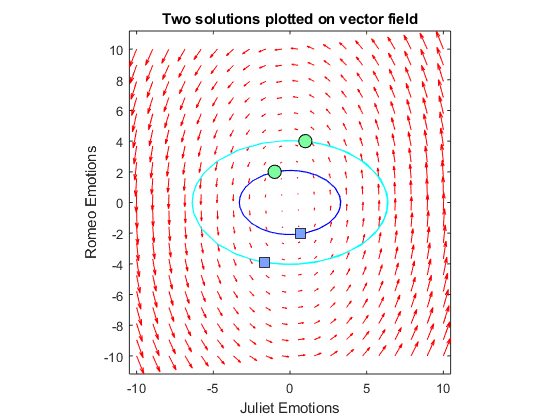
\includegraphics[width=0.5\linewidth]{RomeoJuliet.png}
    \caption{Vector field of the Romeo and Juliet set of differential equations}
    \label{fig:RJ}
\end{figure}
We can also take a look at the Lotka-Volterra model which describes predator-prey dynamics and is described by the equations 
\begin{equation*}
    \begin{split}
        \dot x&= x-kxy \\
        \dot y&=kxy-y
    \end{split}
\end{equation*}
We can see that in Figure \ref{fig:LV}, there exists a fixed point at the origin (no predators and no prey so no dynamics) and another one somewhere in the positive plane which suggests the existence of a steady state.
\begin{figure}[htbp]
    \centering
    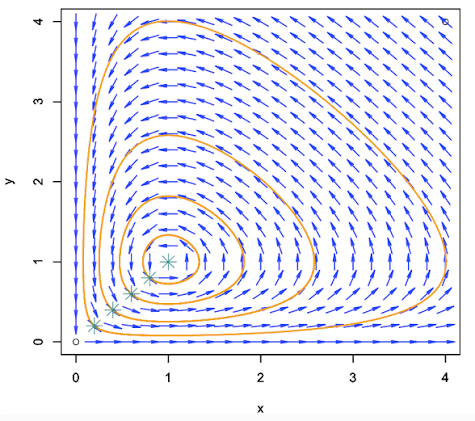
\includegraphics[width=0.5\linewidth]{LotkaVolterra.png}
    \caption{Vector field of the Lotka-Volterra model}
    \label{fig:LV}
\end{figure}

\end{document}
